%%%%%%%%%%%%%%%%%%%%%%%%%%%%%%%%%%%%%%%%%%%%%%%%%%%%%%%%5
% basis specials
%%%%%%%%%%%%%%%%%%%%%%%%%%%%%%%%%%%%%%%%%%%%%%%%%%%%%%%%5
% make "impressive" work (only with pdf version 4..)
\pdfminorversion=4

% choose between handout format and beamer format.
\documentclass[t,handout,xcolor={dvipsnames,table}]{beamer}
%\documentclass[t,12pt,handout,xcolor=table]{beamer}
%\documentclass[t,xcolor=table]{beamer}

%%%%%%%%%% styling
\usepackage{linuxcursus}
\usepackage{frames}

%%%%%%%%%%%%% Text placement
%\setbeamerfont{block title}{size={}}
\setbeamersize{text margin left=1.5cm,text margin right=1cm}
\setbeamertemplate{frametitle}{\insertframetitle\vskip-11pt\vskip15pt\hfill\usebeamerfont{framesubtitle}\insertframesubtitle\vskip-24pt\hrulefill}

\setbeamerfont{section in toc}{size=\tiny}
\setbeamerfont{subsection in toc}{size=\tiny}
\renewcommand{\ttdefault}{pcr}

%%%%%%%%%% description list
% align left with our description list
\defbeamertemplate{description item}{align left}{\insertdescriptionitem\hfill}
\setbeamertemplate{description item}[align left]

%%%%%%%%%%% blocks
% round corners for blocks
\setbeamertemplate{blocks}[rounded][shadow=false]
% block title color, fonts in section/subsection in toc
\setbeamercolor{block title}{use=structure,fg=kwalinux}
% set example block color
%\setbeamercolor*{block body example}{fg= blue, bg= blue!5}

%%%%%%%%%%% special chars, html entities
%\newcommand{\Ent}[1]{\char#1 }
% for |, >, <
\usepackage[T1]{fontenc}
% \ding{nummer}, bv 122 = zwarte cursor
\usepackage{pifont}
% more specials: \Enter etc..
\usepackage{keystroke}
% \frown (not working?)
%\DeclareMathAlphabet\mathbb{U}{msb}{m}{n}
%\usepackage{MnSymbol}
% smilies
\usepackage{wasysym}

% for Verbatim / terminal
\usepackage{fancyvrb,listings}
%\lstdefinestyle{terminal}{basicstyle=\ttfamily}
\newenvironment{terminal}[1][]
  { \VerbatimEnvironment%
    \begin{Verbatim}[#1]}
  { \end{Verbatim}  }

% frame with border
%\fvset{frame=single,framesep=1mm,fontfamily=courier,fontsize=\scriptsize,framerule=.2mm,numbersep=1mm,commandchars=\\\{\}}

%%%%%%%%%%%%%%% % for terminal examples
\usepackage{tcolorbox}
\tcbset{%
    noparskip,
    colback=gray!10, %background color of the box
    colframe=gray!40, %color of frame and title background
}

% translate
\usepackage[dutch]{babel}

% textblocks positioning
%\usepackage[absolute,overlay]{textpos}

%%%%%%%%%%%%%%% drawing
\usepackage{tikz}
% extra for trees (filesystem..)
\usepackage{tikz-qtree}
\usetikzlibrary{arrows, shapes, backgrounds}
\tikzstyle{startstop} = [rectangle, rounded corners, minimum width=3cm, minimum height=1cm,draw=black, fill=black!30, text width=3cm]
\tikzstyle{process} = [rectangle, minimum width=0cm, minimum height=0cm, text centered, draw=black, fill=white, text width=1cm]
\tikzstyle{button} = [minimum width=0cm, minimum height=0cm, text centered, fill=white, text width=1cm]
\tikzstyle{every node}=[font=\small]
%\tikzstyle{arrow} = [thick,->,>=stealth]
% apply the 'remember picture' style. To avoid some typing, we'll apply
% the style to all pictures.
% this is to point correctly from a -> b (with nodes and arrows)
\tikzstyle{every picture}+=[remember picture]
% By default all math in TikZ nodes are set in inline mode. Change this to
% displaystyle so that we don't get small fractions.
\everymath{\displaystyle}


%%%%%%%%%%% more packages
% include pictures
\usepackage{graphicx}
% make columns
\usepackage{multicol}
% ???
\usepackage{booktabs}
%\usepackage{parskip}
%\setlength{\parskip}{\smallskipamount} 
%%%%%%%%%%%%%%%%%%%%%%%%%%%%%%%%%%%%%%%%%%%%%%%%%%%%%%%%5
\title{SELinux}
%\subtitle{}
\author{Oscar Buse\\
{\small 9 juni 2015\\
NLUG}}

\date{}

%%%%%%%%%%%%%%%%%%%%%%%%%%%%%%%%%%%%%%%%%%%%%%%%%%%%%%%%5
\begin{document}
\setbeamertemplate{navigation symbols}{}
\setbeamertemplate{section in toc}[ball unnumbered]
\setbeamertemplate{subsection in toc}[default]
    \begin{sectionframe}
        \titlepage
    \end{sectionframe}

%    \begin{sectionframe}
%    \frametitle{Inhoudsopgave}
%\vspace{-14pt}
%    \fontsize{6}{9}\selectfont
%    \begin{columns}[t]
%        \begin{column}{.5\textwidth}
%                \begin{block}{}
%                        \tableofcontents[sections={1-3}]
%                        \tableofcontents[sections={4-6}]
%                \end{block}
%        \end{column}
%    \end{columns}
%    \end{sectionframe}

    \section{Inleiding}
\subsection{}
\begin{styleframe}
	\frametitle{Inleiding}
Dit praatje gaat over docker: een Linux container technologie.

De onderwerpen die aan bod komen:
\begin{itemize}
	\item Waarom docker?
	\item Wat is docker?
	\item Installatie.
	\item De docker omgeving.
	\item Images, layers en containers..
	\item Enkele praktijk voorbeelden I.
	\item Enkele veel gebruikte commando's.
	\item cgroups en namespaces.
	\item Praktijk voorbeeld 4.
	\item Linking containers
	\item Troubleshooting.
	\item Uploaden van je container/image naar een repository.
	\item De voor- en nadelen van docker.
	\item Best practices
\end{itemize}
\end{styleframe}

\section{Waarom docker?}
\subsection{}
\begin{styleframe}
	\frametitle{Waarom docker?}
\begin{itemize}
	\pause
	\item ''Op mijn development omgeving werkt alles prima!'' \pause Docker: ''{\it build once, run anywhere}''
	\pause
	\item Kleine {\it footprint} en mede daardoor:
	\begin{itemize}
		\item goed schaalbaar.
		\item snelle startup.\\
	\end{itemize}
	\pause
	In een zeer versimpelde weergave:\\
~\\
	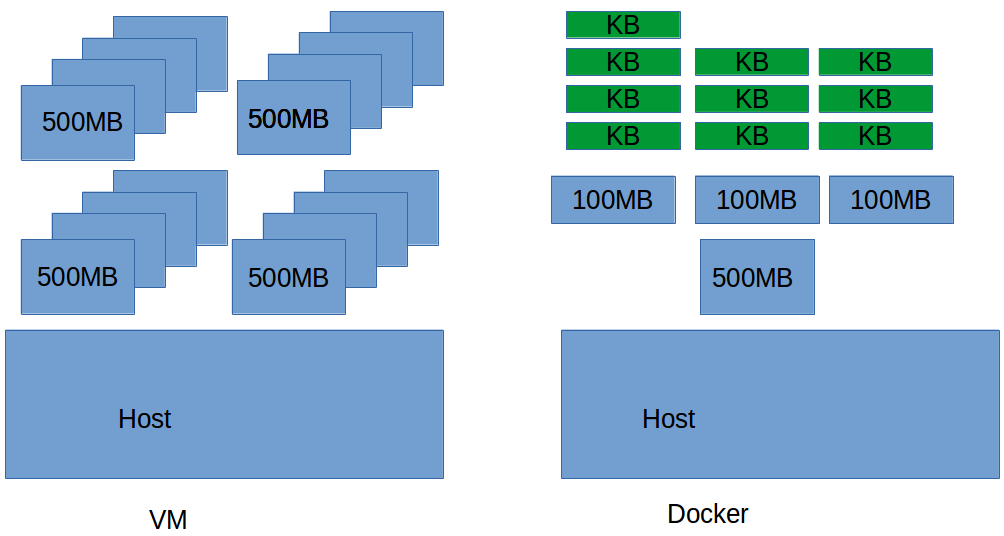
\includegraphics[width=9cm]{img/VM_vs_Docker.png}\\
\end{itemize}
\end{styleframe}

\section{Wat is docker?}
\subsection{}
\begin{styleframe}
	\frametitle{Wat is docker? 1/2}
\pause
Zomaar wat eigenschappen van docker containers:
\begin{itemize}
	\item Vrij nieuw: 15/03/2013. Flink groeiende user-base.
	\pause
	\item Container technologie (denk aan OpenVZ, LXC, Solaris zones, ...)
	\pause
	\item Denk meer aan een single proces dan aan een VM.
	\pause
	\item Verspreidbare (software) eenheid voor elke omgeving (als er maar een docker daemon runt). Handig voor software workflows (OTAP).
	\pause
	\item ''Build once, run anywhere''.
	\pause
	\item Vluchtig: meer geschikt voor een kortdurend bestaan (maar hoeft niet). Bv. volstrekt normaal om docker eenmalig een extern reguest te laten doen (later meer). 
	\pause
	\item Meer geschikt voor stateless applicaties.
\end{itemize}
\end{styleframe}

\subsection{}
\begin{styleframe}
	\frametitle{Wat is docker? 2/2}
\begin{itemize}
	\item Goed voor ''microservices'' (grote applicatie opgedeeld in kleinere delen (microservices)).
	\pause
	\item Zuinig met diskruimte: {\it images} worden geshared.
	\pause
	\item Snelle startup (voor bv. bijschakelen resources (denk bv. aan extra webservers)).
	\pause
	\item ''Een {\it image} voor iedere toepassing'' (in de repositories).
\end{itemize}
\end{styleframe}

\section{Installatie}
\subsection{}
\begin{styleframefrag}
	\frametitle{Installatie}
Docker heeft zijn {\bf eigen} repository voor het package ''docker-engine''.\\
\pause
~\\
Voor bv. CentOS:
{\tiny
\begin{verbatim}
    # yum install -y yum-utils
    # yum-config-manager --add-repo \
        https://docs.docker.com/engine/installation/linux/repo_files/centos/docker.repo
    Daarna: install, update (downgrade) docker vanuit de repositorie:
    # yum install docker-engine
(alternatief: curl -sSL httpd://get.docker.com | sh)
\end{verbatim}
}
\pause
Test bv. met ''docker run hello-world''
\end{styleframefrag}

\subsection{}
\begin{styleframe}
	\frametitle{De docker omgeving}
Een overzicht:
\begin{itemize}
	\item dockerd - de docker daemon
	\pause
	\item docker - de cli
	\pause
	\item remote API
	\pause
	\item repositories met docker images (hub.docker.com)
	\pause
	\item compose, machine (voor docker hosts), swarm, k8s ({\it orchestration}, volgende keer).
	\pause
\end{itemize}
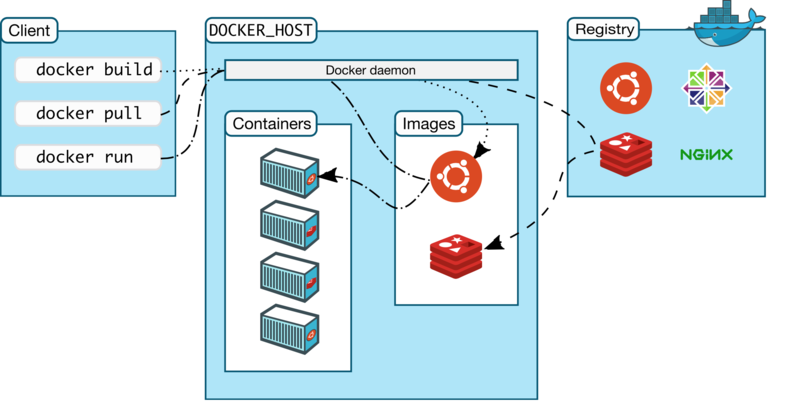
\includegraphics[width=9cm]{img/docker.png}\\
\end{styleframe}

\section{Theorie}
\subsection{}
\begin{styleframe}
	\frametitle{Images, layers en containers.. 1/2}
Voordat we een praktijkvoorbeeld zien eerst wat meer over images, layers en containers..:
\pause
\scriptsize
\begin{description}[containerbla]
	\item[image] Filesysteem als read-only basis voor een container.  Bestaat uit meerdere (ook read-only) layers. {\it Distributable unit}.
	\pause
	\item[layers] ''Filesysteem verandering in een image''. De docker storage engine combineert meerdere layers tot 1 view (filesysteem) met {\it union mounting}.
	\pause
	\item[container] Docker image met een dunne schrijfbare laag toegevoegd.
	\pause
\end{description}
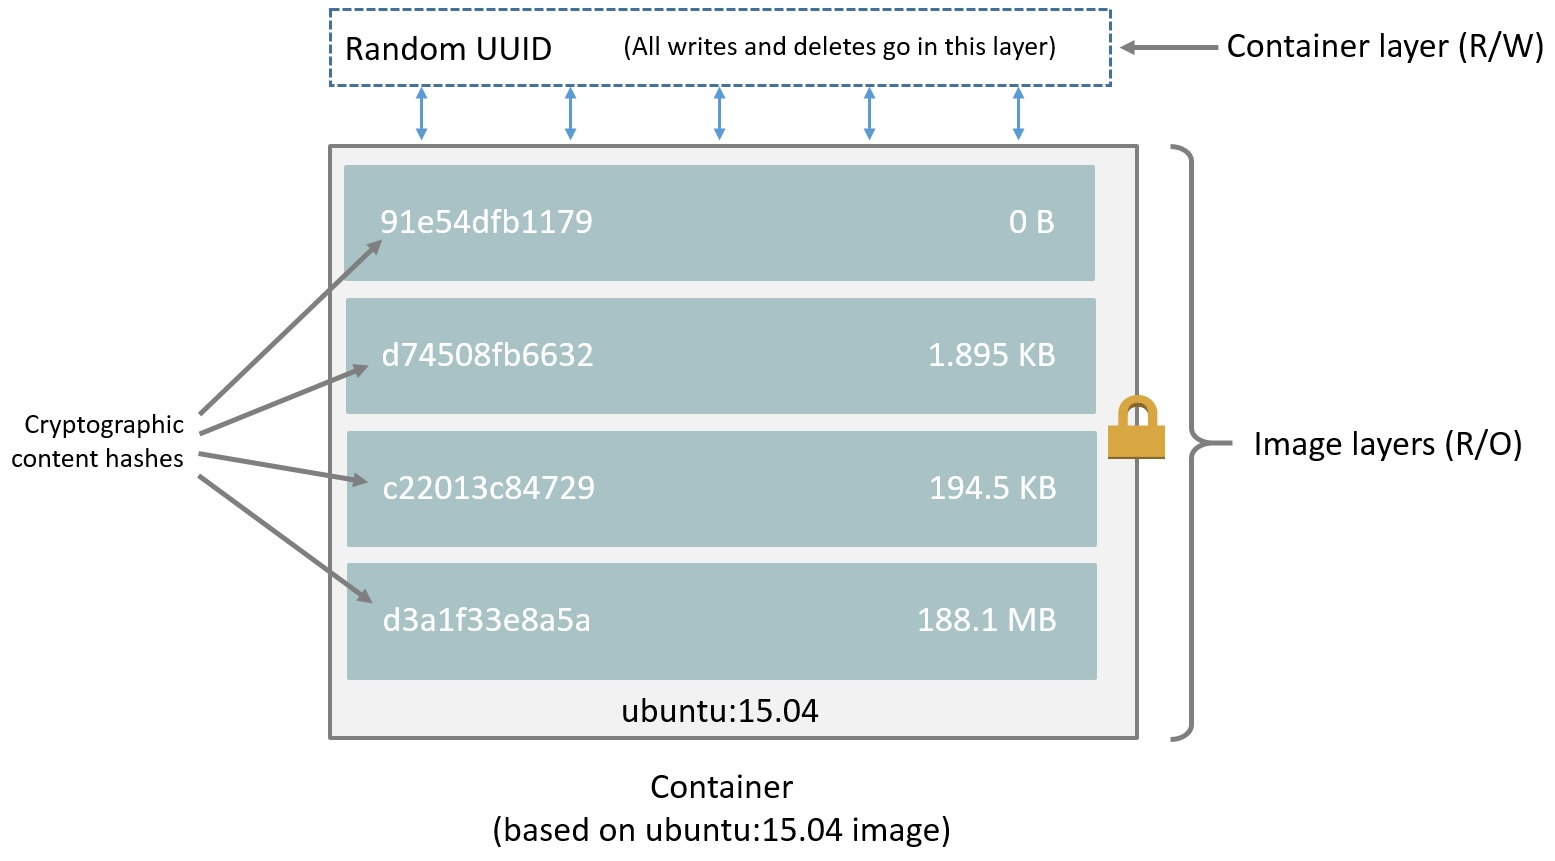
\includegraphics[width=9cm]{img/container-layers-cas.jpg}\\
\end{styleframe}

\subsection{}
\begin{styleframe}
	\frametitle{Images, layers en containers.. 2/2}
\begin{itemize}
	\item Sharen van image layers: zuinig mbt diskusage, \pause performance winst.
	\pause
	\item Copy-on-Write (CoW) toegepast.
	\pause
	\item V\'{o}\'{o}r versie 1.10: layers en images opgeslagen met random UUID. Nadelen hiervan:
	\pause
	\begin{description}[min]
		\item[-] slechte data integriteit (geen checksums). Vanaf v1.10  sha256 voor layers en images.
		\pause
		\item[-] kans op dubbele ID's.
%		\item[-] layers/images minder goed te sharen (vooral tussen verschillende builds).
	\end{description}
\end{itemize}
\end{styleframe}

\subsection{}
\begin{styleframe}
    \frametitle{cgroups en namespaces}
Docker maakt gebruik van cgroups en namespaces:
\pause
\begin{description}[namespacesbla]
	\item[cgroups] Limit resources.
	\pause
	\begin{itemize}
		\item iedere container eigen cgroup (onder /sys filesystem).
% niet persistent. Wel vanaf v1.6 create custom cgroup outside docker and attach a new container to it.
	\end{itemize}
	\pause
	\item[namespaces] Gelijke namen mogelijk door isolatie van de namespace. Enkele voorbeelden:
	\begin{itemize}
		\pause
		\item mount namespace (bv. / in container != / in host != / in andere container)
		\pause
		\item PID namespace
		\pause
		\item Netwerk namespace - (bv. port 80 in container != port 80 on host)
		\pause
		\item User namespace - root heeft bv. wel eigen namespace maar ja.. 
	\end{itemize}
\end{description}
\end{styleframe}

\section{Praktijk}
\subsection{}
\begin{styleframefrag}
    \frametitle{Enkele praktijk voorbeelden I}
Algemene werkwijze met docker containers:
\begin{itemize}
	\pause
	\item build (maak een image mbv een Dockerfile)
	\begin{itemize}
		\pause
		\item \verb!docker build -t voorbeeld/mijn_image .!
	\end{itemize}
	\pause
	\item run (= create + start container van image)
	\begin{itemize}
		\pause
		\item \verb!docker run voorbeeld/mijn_image!
	\end{itemize}
\end{itemize}
\pause
Voorbeeld 1: Hello world\\
\pause
Voorbeeld 2: Een random quote\\
\pause
~\\
Voorbeeld 3: Nog een random quote (\url{https://github.com/oscarbuse/quote-web})\\
\end{styleframefrag}

\subsection{}
\begin{styleframefrag}
	\frametitle{Enkele veel gebruikte commando's}
Maken/Verkrijgen van een image:
\pause
\begin{itemize}
	\item Custom mbv ''Dockerfile'': \verb!# docker build!
	\pause
	\item Downloaden met: \verb!# docker pull!
	\pause
\end{itemize}
Enkele commando's:
\tiny
\begin{itemize}
	\item \verb!docker version! (tegenwoordig in YY.MM format ({\it monthly release cycle}))
	\pause
	\item \verb!docker info | less!
	\pause
	\item \verb!docker build -t example/quote-web .!
	\pause
	\item \verb!docker pull <image van reposotory>!
	\pause
	\item \verb!docker run -d -m 500m --rm --read-only --name quote-web \!
		  \verb!           -p 8081:8080 example/quote-web!
	\pause
	\item \verb!docker images!
	\pause
	\item \verb!docker ps!
	\pause
	\item \verb!docker stop <CONTAINER\_ID/NAME>! (stop container)
	\pause
	\item \verb!docker stop $(docker ps -a -q)! (stop alle containers)
	\pause
	\item \verb!docker rm <CONTAINER\_ID/NAME>! (remove container)
	\pause
	\item \verb!docker rmi <IMAGE\_ID>!  (remove image)
	\pause
	\item \verb!docker exec -it quote-web /bin/bash! (krijg een shell in de container ''quote-web'')
	\pause
\end{itemize}
%Praktijk:
%    install Docker software for your platform
%    run a software image in a container
%    browse for an image on Docker Hub
%    create your own image and run it in a container
%    create a Docker Hub account and an image repository
%    create an image of your own
%    push your image to Docker Hub for others to use
% examples
%docker run -dit -P --name web -v /var/stack/docker/d1:/web1:z changed-ubuntu bash
%Commando's mbt containers
%Commando's mbt images
%Docker usage (commands)
\end{styleframefrag}

\subsection{}
\begin{styleframefrag}
    \frametitle{Praktijk voorbeeld 4}
Voorbeeld 4: 2 containers in een apart subnet (\url{https://github.com/oscarbuse/hours}).\\
\pause
Enkele commando's:
\tiny
\begin{itemize}
	\item \verb!docker network create --subnet=172.18.0.0/16 hours-net!
	\pause
	\item \verb!docker network ls! (toont alle netwerken)
	\pause
	\item \verb!docker run -d --net hours-net --ip 172.18.0.3 -p 8010:8080\!\\
          \verb!           --name web oscarbuse/hours-web!
	\pause
	\item \verb!docker run -d --net hours-net --ip 172.18.0.2 --name db\!\\
		  \verb!           -v /var/lib/mysql:/var/lib/mysql example/hours-db!
\end{itemize}
\end{styleframefrag}

\subsection{}
\begin{styleframefrag}
    \frametitle{Linking containers}
\pause
Containers zijn eenvoudig te linken door naar de naam te verwijzen. Je hoeft dan geen eigen subnet te cre\"{e}eren.\\
\pause
~\\
Een voorbeeld van een Wordpress container gelinkt met een MySQL database container:
\tiny
\begin{itemize}
	\item \verb!docker pull wordpress:latest!
	\item \verb!docker pull mysql:latest!
	\item \verb!docker run --name mysqlwp -e MYSQL_ROOT_PASSWORD=changeme -d mysql!
	\item \verb!docker run --name wordpress --link mysqlwp:mysql -p 8080:80 -d wordpress!
	\item \verb!docker ps!
\end{itemize}
\pause
~\\

\small
Met joomla:
\tiny
\begin{itemize}
	\item \verb!docker pull joomla:latest!
	\item \verb!docker run --name joomla --link mysqlwp:mysql -p 8081:80 -d joomla!
	\item \verb!docker ps!
\end{itemize}

\end{styleframefrag}

\subsection{}
\begin{styleframefrag}
    \frametitle{Troubleshooting}
\begin{itemize}
	\pause
	\item \verb!docker logs <CONTAINER\_ID/NAME>!
	\pause
	\item \verb!docker exec -it <CONTAINER\_ID/NAME> bash!
	\pause
	\item \verb!docker inspect <CONTAINER\_ID/NAME>!
	\pause
	\item \verb!docker stats! (monitoring)
	\pause
	\item \verb!docker events!
	\pause
	\item \verb!docker diff! (handig voor read-only maken)
	\pause
	\item \verb!docker volume prune! (opruimen, bespaar diskruimte)
\end{itemize}
\pause
Monitor je containers.\\
\pause
Verschillende tools mogelijk:
\begin{itemize}
	\pause
	\item cAdvisor (geen alerting)
	\pause
	\item Prometheus (wel alerting)
	\pause
	\item Scout, Datadog (hosted, wel alerting, kost geld)
	\item ...
	\pause
\end{itemize}
Waarschijnlijk goed om de monitoring te integeren in een gemanagede container omgeving (volgende keer meer).
\end{styleframefrag}

\subsection{}
\begin{styleframefrag}
    \frametitle{Up/downloaden van je container/image naar een repository.}
\begin{itemize}
	\pause
	\item \verb!docker login!
	\pause
	\item \verb!docker push oscarbuse/hours-web!
	\pause
	\item \verb!docker pull oscarbuse/hours-web!
\end{itemize}
\pause
Bij een gewijzigde container eerst: \verb!docker commit <container_id/name> <image name>!
\end{styleframefrag}


\section{Concluderend}
\subsection{}
\begin{styleframe}
    \frametitle{Voordelen}
\scriptsize
\begin{description}[plus]
    \item[+] Geen dependency issues ("but it worked on my development environment..??").
    \pause
    \item[+] Geen conflicten, isolatie van software.
    \pause
    \item[+] Makkelijk OTAP mogelijk.
    \pause
    \item[+] Lichtgewicht, lage overhead.
    \pause
    \item[+] CLI (docker) en web API.
    \pause
    \item[+] Meer richting een {\it immutable} omgeving. CM (Configuration Management) groeit in complexiteit.
    \pause
    \item[+] Goed te gebruiken als virtualisatie op virtualisatie: bv. docker containers in een kvm guest. Of in een aws/google omgeving.
    \pause
    \item[+] grote userbase, veel standaard tooling.
    \pause
    \item[+] Goede integratie met andere tooling (voor CI/CD)
    \pause
\end{description}
\end{styleframe}

\subsection{}
\begin{styleframefrag}
    \frametitle{Nadelen}
\pause
\scriptsize
\begin{description}[plus]
    \item[-] Security..
		\pause
		\begin{itemize}
			\item dockerd is (extra) root proces.
			\item root in container <-> root op host (..): alleen scheiding door gebruik van namespaces.\\
\pause
Dit kun je opvangen door de docker daemon te starten met --userns-remap=default:
\begin{verbatim}
# cat << 'EOF' >> /etc/systemd/system/docker.service.d/userns-remap.conf
[Service]
ExecStart=
ExecStart=/usr/bin/dockerd --userns-remap=default -H fd:// $DOCKER_OPTS
EOF
# systemctl daemon-reload
# systemctl restart docker.service
\end{verbatim}
			\pause Creert wel nieuwe images!
			\pause
			\item Zorg dat processen in de container niet als root runnen.
			\pause
			\item Run dockerd in een dedicated VM.
		\end{itemize}
    \pause
    \item[-] Docker bepaald eigenschappen van de container tijdens het bouwen. Het monitort/managed niet.
    \pause
    \item[-] Ongebruikte images/volumes kan veel zijn en dient opgeruimd te worden.
    \pause
    \item[-] Docker daemon alleen voor Linux.
    \pause
    \item[-] Minder geschikt voor {\it stateful} applicaties (bv. databases).
    \pause
    \item[-] Default geen limiet op resources.
    \pause
    \item[-] T\'{e} dominant?
\end{description}
\end{styleframefrag}

\subsection{}
\begin{styleframefrag}
    \frametitle{Best practices}
\begin{itemize}
	\item pas op met ''latest''.
	\pause
	\item pas op met \verb!apt-get update! (duurt lang).
	\pause
	\item beperk container interactie (focus op container interactie onderling).
	\pause
	\item denk aan patching/upgrading van de ''base'' images.
	\pause
	\item pas read-only toe waar mogelijk.
	\pause
	\item gebruik TLS voor remote connectie met de docker daemon.
	\pause
	\item focus op stateless.
	\pause
	\item hou het simpel (iedere container specifieke taak, containers combineren met linking).
	\pause
	\item monitor.
\end{itemize}
\end{styleframefrag}

\subsection{}
\begin{styleframe}
    \frametitle{Referenties}
\begin{itemize}
	\item \url{https://www.google.com}
	\item \url{https://www.docker.com}
	\item \url{https://docs.docker.com}
	\item \url{https://www.digitalocean.com/community/tutorials/how-to-install-and-use-docker-on-ubuntu-16-04}
	\item \url{https://hub.docker.com}
	\item Voorbeeld 3: \url{https://github.com/oscarbuse/quote-web}
	\item Voorbeeld 4: \url{https://github.com/oscarbuse/hours}
\end{itemize}
\end{styleframe}

\subsection{}
\begin{styleframe}
    \frametitle{Vragen?}
\begin{center}
\hspace{-20pt} \Huge Bier?
\end{center}
\end{styleframe}

%	\section{Werkwijze en tooling}
\begin{frame}
    \frametitle{Configuratie}
\begin{itemize}
\pause
\item  hoe weet je nu wat een huidige policy is? -> \pause sesearch
\pause
{\tt sesearch -Ad -s httpd\_t -t httpd\_sys\_content\_t -c file}
Verder spitten met: seinfo -ahttpdcontent -x
\item niet zo interessant: bestaande policies hebben goede defaults.
\item wel interessant: wat als je de policy wilt aanpassen of toevoegen? 
semodule_unpackage: maar niet de bedoeling dat je de default policies wijzigt...wordt ontmoedigt
semanage: config policies zonder de default policy te wijzigen. Straks meer
\end{itemize}
\end{frame}

\section{Voorbeeld scenario}
\begin{frame}
    \frametitle{BackupPC}
BackupPC is een handige grafische schil om rsync voor het maken van backups.
Er is geen standaard policy voor dus die moeten we zelf maken. \\
De stappen:
\footnotesize
\begin{itemize}
\item definieer de file context (fc): in dit geval httpd\_sys\_content\_t \\
Commando's: \\
{\tt \# semanage fcontext -a -t httpd\_sys\_content\_t  \\
\hspace{7pt} '/vol-thishost-1/BackupPC/pc(/.*)?' \\
\# restorecon -Rv /vol-thishost-1/BackupPC/pc \\
\# semanage fcontext -a -t httpd\_log\_t \\
\hspace{7pt} '/var/log/BackupPC(/.*)?' \\
\# restorecon -Rv /var/log/BackupPC/}
\item Kijk naar denied regels in /var/log/audit/audit.log en stop in file -> backuppc.txt
\item Maak van opgespaarde denied regels in file policy rules (met audit2allow): \\
{\tt cat backuppc.txt  | audit2allow -M backuppc} geeft:
	\begin{itemize}
	\item De Type Enforcement rules (ascii): backuppc.te
	\item Het binaire policy file met de type enforcement allow rules: backuppc.pp
	\end{itemize}
\item De nieuwe policy rules 
\item {\tt \# semodule -i backuppc.pp}
\item 
Dit geeft ook een .te file (ascii, Type Enforcement rules)
\bf{Let op:} niet alles wordt standaard gelogt...
\end{itemize}
\end{frame}

\end{document}
